% LinEnvLearn-PAMI-2013
% Stephen Gould <stephen.gould@anu.edu.au>
%
% Contributions over ICML paper:
% 1. re-introduce per-variable weight w_i
% 2. observation that b_1 = 0 without loss of generality
% 3. lemma that constraints on z_k are not required
% 4. proof for polynomial time max-margin convergence
% 5. more synthetic experiments comparing different formulations
% 6. Weizmann horses experiments

\documentclass[10pt,journal,letterpaper,compsoc]{IEEEtran}

% For figures
% \ifCLASSINFOpdf
\usepackage[pdftex]{graphicx}
\DeclareGraphicsExtensions{.jpg,.png}
%\else
%\usepackage[dvips]{graphicx}
%\DeclareGraphicsExtensions{.eps}
% \fi

% For citations
%% \ifCLASSOPTIONcompsoc
%% \usepackage[nocompress]{cite}
%% \else
%% \usepackage{cite}
%% \fi

\usepackage[sort,numbers]{natbib}
\renewcommand{\citename}{\citet}
\renewcommand{\cite}{\citep}
\usepackage{natbibspacing}

% For maths
\usepackage[cmex10]{amsmath}
\usepackage{amssymb,amsthm}

% For algorithms
\usepackage{algorithm}
\usepackage{algorithmic}

% For Hyperlinks
\usepackage{hyperref}
% fix problem between hyperref and algorithmic
\newcommand{\theHalgorithm}{\arabic{algorithm}}

% For captions
\usepackage[font=small,labelfont=bf]{caption}
\usepackage[font=footnotesize]{subfig}

% My macros
\usepackage{sg-macros}

\newtheorem{thm}{Theorem}[section]
\newtheorem{cor}[thm]{Corollary}
\newtheorem{lem}[thm]{Lemma}
\newtheorem{prop}[thm]{Proposition}
\newtheorem{obs}[thm]{Observation}
\newtheorem{defn}[thm]{Definition}

\newcommand{\mmqp}[3]{\textrm{\sc MaxMarginQP}\!\left(\{\by_t, #1\}_{t=1}^{T}, #2, #3\right)}

% correct bad hyphenation here
\hyphenation{op-tical net-works semi-conduc-tor}

\begin{document}

\title{Learning Weighted Lower Linear Envelope Potentials in Binary
  Markov Random Fields}

\author{Stephen~Gould,~\IEEEmembership{Member,~IEEE}%
\IEEEcompsocitemizethanks{\IEEEcompsocthanksitem S.~Gould is with the Research
School of Computer Science, Australian National University, ACT 0200, Australia.\protect\\
E-mail: stephen.gould@anu.edu.au}%
\thanks{}}


% Abstract -------------------------------------------------------------------------

\IEEEcompsoctitleabstractindextext{%
  \begin{abstract}
    Markov random fields containing higher-order terms are becoming
    increasingly popular due to their ability to capture complicated
    relationships as soft constraints involving many output random
    variables. In computer vision an important class of constraints
    encode a preference for label consistency over large sets of
    pixels and can be modeled using higher-order terms known as
    \emph{lower linear envelope potentials}. In this paper we develop
    an algorithm for learning the parameters of binary Markov random
    fields with weighted lower linear envelope potentials. We first
    show how to perform exact energy minimization on these models in
    time polynomial in the number of variables and number of linear
    envelope functions. Then, with tractable inference in hand, we
    show how the parameters of the lower linear envelope potentials
    can be estimated from labeled training data within a max-margin
    learning framework. We explore three variants of the lower linear
    envelope parameterization and demonstrate results on both
    synthetic and real-world problems.
  \end{abstract}
  
  \begin{keywords}
    higher-order MRFs, lower linear envelope potentials, max-margin
    learning
  \end{keywords}
}

% make the title area
\maketitle

\IEEEdisplaynotcompsoctitleabstractindextext
\IEEEpeerreviewmaketitle

% Introduction ---------------------------------------------------------------------
\section{Introduction}
\label{sec:intro}

\IEEEPARstart{M}{arkov} random field (MRF) parameter learning is a
challenging task that has advanced considerably in the past several
years with the introduction of the max-margin principle for structured
prediction~\cite{Tsochantaridis:ICML04, Taskar:ICML05}. The standard
max-margin approach is to learn model parameters by constraining the
prediction rule to favour the ground-truth assignment over all other
joint assignments to the variables. Since the set of all possible
joint assignments can be prohibitively large (exponential in the
number of the variables), constraints are introduced incrementally by
finding the most violated ones (with respect to the current parameter
settings) during each iteration of the learning algorithm.

Despite this advance, learning the parameters of an MRF remains a
notoriously difficult task due to the problem of finding the most
violated constraints, which requires performing exact maximum
a-posteriori (MAP) inference. Except in a few special cases, such as
tree-structured graphs or binary pairwise MRFs with submodular
potentials~\cite{Koller:2009}, exact inference is intractable and the
max-margin framework cannot be applied. When substituting approximate
inference routines to generate constraints, the max-margin framework
is not guaranteed to learn the optimal parameters and often performs
poorly~\cite{Finley:ICML08}.

Recently, models with structured higher-order terms have become of
interest to the machine learning community with many applications in
computer vision, particularly for encoding consistency constraints
over large sets of pixels, \eg \cite{Rother:CVPR09, Nowozin:CVPR09,
  Lempitsky:ICCV09}. A rich class of higher-order models, known as
\emph{lower linear envelope potentials}, was proposed
by~\citename{Kohli:CVPR10}. The class defines a concave function of
label cardinality (\ie number of variables taking each label) and
includes the generalized Potts model~\cite{Kohli:CVPR07} and its
variants. While efficient approximate inference algorithms based on
message-passing or move-making exist for these models, parameter
learning remains an unsolved problem.

In this paper we focus on learning the parameters of weighted lower
linear envelope potentials for binary MRFs. We present an exact MAP
inference algorithm for these models that is polynomial in the number
of variables and number of linear envelope functions. This opens the
way for max-margin parameter learning. However, to encode the
max-margin constraints we require a linear relationship between model
parameters and the features that encode each problem instance.

Our key insight is that we can represent the weighted lower linear
envelope in two different ways. The first way encodes the envelope as
the minimum over a set of linear functions and admits tractable
algorithms for MAP inference, which is required during constraint
generation. The second representation encodes the envelope by linearly
interpolating between a sequence of sample points. This representation
allows us to treat the potential as a linear combination of features
and weights as required for max-margin parameter learning. By mapping
between these two representations we can learn model parameters
efficiently. Indeed, other linear parameterizations are also possible
and we explore these together with the corresponding feature
representations.

We evaluate our approach on synthetic data as well as two real-world
problems---a variant of the ``GrabCut'' interactive image segmentation
problem~\cite{Rother:SIGGRAPH04} and segmentation of horses from the
Weizmann Horse dataset~\cite{Borenstein:ECCV02}. Our experiments show
that models with learned higher-order terms can result in improved
pixelwise segmentation accuracy.

% Background -----------------------------------------------------------------------
\section{Related Work}
\label{sec:background}

Our work focuses on a class of higher-order potentials known as lower
linear envelope potentials, which can be used to represent arbitrary
concave functions over the number of variables (in a clique) taking a
given assignment. \citename{Kohli:CVPR10} show how such potentials can
be represented in an energy-minimization setting by introducing a
multi-valued auxiliary variable to select each linear function in the
envelope. In principle, the optimal assignment can be found by jointly
minimizing the energy function over the original variables and this
auxiliary variable. However, this is non-trivial, in general, and
\citename{Kohli:CVPR10} only show how the resulting energy function
can be approximately optimized.

Earlier research, on MRFs with restricted variants of the lower linear
envelope potential, showed how exact inference can be performed in the
binary case. \citename{Kohli:CVPR07} introduced the $P^n$-model for
encoding consistency constraints. This was later extended to the
robust $P^n$-model by \citename{Kohli:TR08} who also describe an
efficient move-making inference algorithm based on
graph-cuts~\cite{Boykov:ICCV99, Boykov:PAMI04}. The robust $P^n$-model
is a lower linear envelope potential with only two terms per
label---one increasing and one constant. Multiple robust $P^n$-models
can be added to form a non-decreasing concave envelope. However, these
works did not address the problem of parameter
learning. \citename{Ladicky:ICCV09} used this model for improving the
quality of multi-class image labeling with parameters set by hand. The
model is still considered state of the art for the multi-class image
labeling task (\ie dense semantic segmentation). For segmenting large
foreground classes (like those in the PASCAL VOC
Challenge~\cite{PASCAL:VOC:2012}) methods based on proposing
whole-object segments are showing promise (\eg
\cite{Carreira:ECCV12}).

In contrast to these works, we propose an algorithm for exactly
optimizing binary MRFs with \emph{arbitrary} lower linear envelope
potentials and show how to learn their parameters. We extend our
previous work~\cite{Gould:ICML2011} to allow each variable within the
potential to be assigned an arbitrary non-negative weight. Our work
and the previous approaches described above are related to a number of
methods in discrete optimization that transform higher-order or
multi-label energy functions into quadratic pseudo-Boolean functions
(\eg \cite{Ishikawa:PAMI03, Ishikawa:CVPR09, Rother:CVPR09}). These
functions have been studied extensively in the operations research
literature (for a survey see \citename{Boros:MATH02}). Under certain
conditions, the resulting pseudo-Boolean function can be minimized
exactly by finding the minimum-cut in a suitably constructed
graph~\cite{Hammer:1965, Freedman:CVPR05}. Our work and other
graph-cut approaches make use of this result.

More general methods---falling under the class of submodular energy
minimization algorithms---can also be used to optimize binary MRFs
with arbitrary lower linear envelope potentials. These include the
strongly polynomial algorithm of \citename{Orlin:MP2009} for general
submodular functions and the recently proposed submodular flows method
of \citename{Kolmogorov:DAM12} for minimizing the sum of submodular
functions. However, the availability of efficient software
implementations and strong empirical performance of graph-cut
approaches~\cite{Boykov:PAMI04} makes graph-cuts the most appropriate
for our problem.

Our max-margin learning framework is based on the approaches
introduced by \citename{Tsochantaridis:ICML04, Tsochantaridis:JMLR05}
and \citename{Taskar:ICML05}, which have been successfully applied
within many application domains (see \citename{Joachims:ML09} for a
recent survey and the ``1-slack'' reformulation).
\citename{Szummer:ECCV08} showed how this framework could be adapted
to learn pairwise MRF parameters using graph-cuts for
inference. Unlike their approach, our method applies to models with
higher-order terms---specifically, weighted lower linear envelopes.


% Main -----------------------------------------------------------------------------

\section{Lower Linear Envelope MRFs}
\label{sec:inference}

We begin with a brief overview of higher-order Markov random fields
(MRFs). We then introduce the lower linear envelope potential and show
how to perform exact inference in models with these potentials. In
\secref{sec:learning} we will discuss learning the parameters of the
models.

\subsection{Higher-order MRFs}
%
The \emph{energy function} for a higher-order MRF over discrete random
variables $\by = \{y_1, \ldots, y_n\}$ can be written as:
%
\begin{align}
  \energy{\by} &= \underbrace{\sum_{i=1}^{n} \psi^U_i\!(y_i)}_{\textrm{unary}} +
  \underbrace{\sum_{ij \in \E} \psi^P_{ij}(y_i, y_j)}_{\textrm{pairwise}} +
  \underbrace{\sum_{c \in \C} \psi^H_c\!(\by_c)}_{\textrm{higher-order}}
  \label{eqn:energy}
\end{align}
% 
where the \emph{potential} functions $\psi^U_i$, $\psi^P_{ij}$ and
$\psi^H_c$ encode preferences for unary, pairwise and $k$-ary variable
assignments, respectively. The pairwise terms, $\psi^P_{ij}$, also
called \emph{edge potentials}, are usually only defined over a sparse
subset $\E$ of possible variable pairs $(y_i, y_j)$. The latter terms,
$\psi^H_c$, are defined over arbitrary subsets of variables (or
\emph{cliques}), $\by_c = \{y_i : i \in c\}$ where $c \subseteq \{1,
\ldots, n\}$ is a subset of variable indices. When $|c| > 2$ these are
known as \emph{higher-order potentials}. The higher-order potentials
can be defined over multiple overlapping cliques. We denote the set of
all cliques for which a higher-order potential is defined by $\C$.

In this paper, we will be concerned with inference and learning of
higher-order binary MRFs (\ie $y_i \in \{0, 1\}$) with weighted lower
linear envelope potentials. These have been attracting much interest
in computer vision applications for encoding consistency constraints
over large subsets of pixels in an image~\cite{Nowozin:2011,
  Lempitsky:ICCV09, Kohli:CVPR07}. A weighted lower linear envelope
potential over a subset (clique) of binary variables $\by_c$ is a
piecewise linear function defined as the minimum over a set of $K$
linear functions as
%
\begin{align}
  \psi^H_c\!(\by_c) \, &\triangleq \min_{k=1, \ldots, K} 
  \left\{ a_k \sum_{i \in c} w^c_i y_i + b_k \right\}
  \label{eqn:potential}
\end{align}
%
where $w^c_i \geq 0$ are non-negative per-variable weights
for each clique with $\sum_{i \in c} w^c_i = 1$, and $(a_k, b_k) \in
\reals^2$ are the linear function parameters.%
%
\footnote{The condition that $\sum_{i \in c} w^c_i = 1$ is assumed so
  that the same parameters $(a_k, b_k)$ can be used for cliques with
  different per-variable weights and still produce the same shaped
  lower linear envelope. Note that if $Z = \sum_{i \in c} w^c_i \neq
  1$ we can always normalize the $w^c_i$ by dividing throughout by $Z$.}
%
To simplify notation in the sequel, we will define the \emph{weight}
of the clique for a given assignment $\by_c$ as $W_{\!c}(\by_c) =
\sum_{i \in c} w_i y_i$. Using this definition we can
re-write~\eqnref{eqn:potential} as
%
\begin{align}
  \psi^H_c\!(\by_c) \, &= \min_{k=1, \ldots, K} \left\{ a_k W_{\!c}(\by_c) + b_k \right\}.
  \label{eqn:potential2}
\end{align}

Note that if all variables are assigned the same weight $w^c_i =
\frac{1}{|c|}$, then $W_{\!c}(\by_c)$ is simply the proportion of
variables in the clique taking assignment one. This restriction (of
uniform weights) was assumed in \citename{Gould:ICML2011}.

\figref{fig:nonredundant} depicts an example lower envelope for three
linear functions. \citename{Kohli:CVPR10} showed that this
representation can encode arbitrary concave functions of
$W_{\!c}(\by_c)$ given sufficiently many linear functions. The
parameterization, however, is not unique.

\begin{figure}[t]
  \centering
  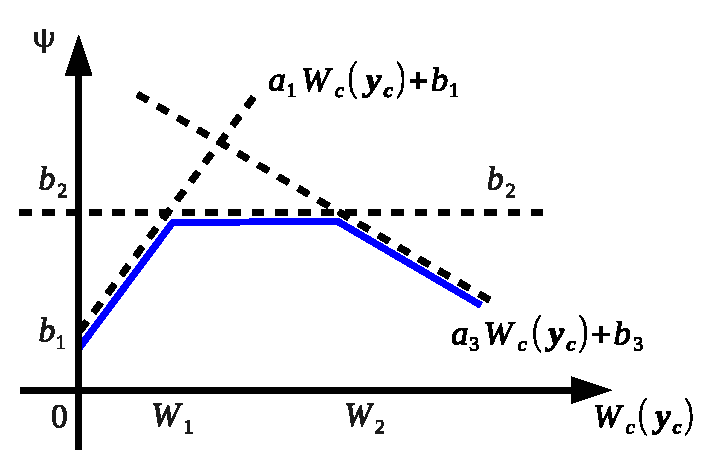
\includegraphics[width=0.8\columnwidth]{figures/not_redundant}
  \caption{\label{fig:nonredundant} Example lower linear envelope
    $\psi^H_c\!(\by_c)$ (shown solid) with three terms (dashed) as a
    function of $W_{\!c}(\by_c) = \sum_{i \in c} w^c_i y_i$.  When
    $W_{\!c}(\by_c) \leq W_1$ the first linear function is active,
    when $W_1 < W_{\!c}(\by_c) \leq W_2$ the second linear function is
    active, otherwise the third linear function is active.}
\end{figure}

\begin{defn}[{\bf Active}]
  We say that the $k$-th linear function is \emph{active} with respect
  to an assignment $\by_c$ if $\psi^H_c\!(\by_c) = a_k W_{\!c}(\by_c)
  + b_k$.
\end{defn}

Note that more than one linear function can be active for the same
assignment (\eg at points where two or more linear functions
intersect). Clearly, however, if a linear function is never active, or
only active whenever another linear function is also active, it can be
removed from the potential without changing the energy function.

\begin{defn}[{\bf Redundant}]
  We say that the $k$-th linear function is \emph{redundant} if it is
  not active for any assignment to $\by_c$ in any clique $c \in \C$ or
  is only active whenever another linear function is also active.
\end{defn}

Although not strictly necessary, in the following, we assume that our
potentials do not contain redundant linear functions. Furthermore, we
assume that the parameters $\{(a_k, b_k)\}_{k=1}^K$ are sorted in
decreasing order of $a_k$. Clearly, this implies that $a_k > a_{k+1}$
and $b_k < b_{k+1}$ since if not then the $k$-th linear function will
lie above the $(k+1)$-th linear function for all configurations of
$\by_c$, \ie the $k$-th linear function will never be active.

One may ask what conditions on $\{(a_k, b_k)\}_{k=1}^K$ ensure that
the potentials do not have any redundant linear functions. The
following proposition provides such a characterization.

\begin{proposition}
  \label{prop:condition}
  Let $f : [0,1] \rightarrow \reals$ be defined by $f(x) =
  \min_{k=1,\ldots,K} \left\{a_k x + b_k\right\}$. Assume the $a_k$
  are sorted in decreasing order (so $a_k > a_{k+1}$). Then the $k$-th
  linear function is not redundant if
  \begin{align}
    0
    <
    \frac{b_k - b_{k-1}}{a_{k-1} - a_k}
    <
    \frac{b_{k+1} - b_k}{a_k - a_{k+1}}
    <
    1.
  \end{align}
\end{proposition}

\begin{proof}
  The $k$-th linear function is active (and no other linear function
  is active) if there exists $x \in (0, 1)$ such that the following
  two inequalities hold
  \begin{align*}
    a_{k-1} x + b_{k-1} &> a_k x + b_k \\
    a_{k+1} x + b_{k+1} &> a_k x + b_k
  \end{align*}
  Rearranging for $x$ and adding the constraint that $0 < x < 1$ gives
  the result.
\end{proof}
\bigskip

Finally, we note that arbitrarily shifting each linear function in the
lower-linear envelope potential up or down by the same fixed constant
does not change the energy-minimizing assignment $\by^\star$ as
captured by the following observation.

\begin{observation}
\label{obs:b0}
Let $\psi^H_c\!(\by_c)$ be defined as in \eqnref{eqn:potential2} and
let $\widetilde{\psi}^{H}_c\!(\by_c) = \min_{k=1, \ldots, K}
\left\{a_k W_{\!c}(\by_c) + b_k + b^\textrm{const} \right\}$. Then
%
\begin{align}
  \argmin_{\by_c} \psi^H_c\!(\by_c)
  &= \argmin_{\by_c} \widetilde{\psi}^{H}_c\!(\by_c).
\end{align}
%
\end{observation}

This property will be useful when considering different learning
algorithms and will allow us to make convenient assumptions such as
$b_1 = 0$ (and therefore all the $b_k$ are non-negative), without loss
of generality.

\subsection{Exact Inference}
\label{sec:exact_inference}

The goal of inference is to find an energy-minimizing assignment
$\by^\star \in \argmin_{\by} \energy{\by}$. As we will show our energy
function is submodular so can be solved in time polynomial in the
number of variables by general-purpose submodular minimization
algorithms~\cite{Kolmogorov:DAM12, Orlin:MP2009}. However, the special
form of the lower linear envelope higher-order terms admits the use of
much faster graph-cut based methods. 

We follow the approach of a number of works that address the problem
of inference in certain classes of higher-order MRFs by transforming
the inference problem to that of minimizing a quadratic pseudo-Boolean
function, \ie pairwise MRF (\eg\cite{Freedman:CVPR05, Ishikawa:CVPR09,
  Boros:MATH02}). For example, \citename{Kohli:TR08} showed that exact
inference can be performed using graph-cuts when the potential is a
concave piecewise linear function of at most three terms (one
increasing, one constant, and one decreasing). Arbitrary concave
functions can be handled by decomposing them into a sum of piecewise
linear functions of two or three terms. \citename{Gould:ICML2011}
showed an alternative graph-cut method for minimizing potentials with
arbitrary many terms. We now develop a weighted version of that
method.

Consider, again the weighted lower linear envelope potential
represented by \eqnref{eqn:potential}. Introducing $K-1$ auxiliary
binary variables $\bz = \left(z_1, \ldots, z_{K-1}\right)$, we define
the quadratic pseudo-Boolean function
%
\begin{multline}
  E^c(\by_c, \bz) = a_1 W_{\!c}(\by_c) + b_1 \\
  {}+ \sum_{k = 1}^{K-1} z_k \left( \left(a_{k+1} - a_k\right) W_{\!c}(\by_c) + b_{k+1} - b_k \right)
  \label{eqn:binary_concave_z}
\end{multline}
%
for a single clique $c \in \C$.

The advantage of this formulation is that minimizing over $\bz$,
subject to some constraints, selects (one of) the active function(s)
from $\psi^H_c\!(\by)$ as we will now show.

\begin{proposition}
\label{prop:minpsi}
Minimizing the function $E^c(\by_c, \bz)$ over $\bz$ subject to
$z_{k+1} \leq z_k$ for all $k$ is equivalent to $\min_{k=1, \ldots, K}
\left\{ a_k W_{\!c}(\by_c) + b_k \right\}$, \ie
\begin{align*}
  \psi^H_c\!(\by_c) &= \min_{\bz : z_{k+1} \leq z_k} E^c(\by_c, \bz).
\end{align*}
\end{proposition}
%
\begin{proof}
  The constraints ensure that $\bz$ takes the form of a vector of all
  ones followed by all zeros. There are $K$ such vectors and for $k =
  \ones^T \bz + 1$ we have $E^c(\by_c, \bz) = a_k W_{\!c}(\by_c) +
  b_k$. Therefore, minimizing over $\bz$ is the same as minimizing
  over $k \in \{1, \ldots, K\}$.
\end{proof}
\bigskip

In \citename{Gould:ICML2011} we showed that the constraints on $\bz$
can be enforced by adding $M z_{k+1} (1 - z_k)$ for $k = 1, \ldots,
K-2$ to the energy function with $M$ sufficiently large. We now show
that it is not necessary to add these terms as the constraints are
either automatically satisfied (with $M = 0$) or violations of the
constraints do not affect the value of the energy function or the
optimal assignment of $\by_c$.

\begin{lemma}
Unconstrained (binary) minimization of the function $E^c(\by_c, \bz)$
over $\bz$ is equivalent to minimization of $E^c(\by_c, \bz)$ subject
to the constraints $z_{k+1} \leq z_k$.
\label{lem:noconstraints}
\end{lemma}

Before proving the lemma, we make two observations.

\begin{observation}
  Assume that for some assignment $\by_c$ we have $a_{k+1} W_c(\by_c) +
  b_{k+1} = a_{k} W_c(\by_c) + b_{k}$. Then, for any assignment to $\bz
  \in \{0, 1\}^{K-1}$, flipping the value of $z_k$ does not change
  $E^c(\by_c, \bz)$.
\end{observation}

\begin{observation}
  For any assignment $\by_c$ such that $\left(a_{k+1} - a_{k}\right)
  W_{\!c}(\by_c) + b_{k+1} - b_k \leq 0$ we have that setting $z_k = 1$ will
  result in a lower energy than setting $z_k = 0$.
\end{observation}

We now proceed with the proof of Lemma~\ref{lem:noconstraints}.

\begin{proof}
  Consider minimizing \eqnref{eqn:binary_concave_z} over $\bz$ for
  fixed $\by_c$. Clearly, from our observations above, $z_k = 1$ if
  $\left(a_{k+1} - a_{k}\right) W_{\!c}(\by_c) + b_{k+1} - b_k <
  0$. Likewise $z_k = 0$ if $\left(a_{k+1} - a_{k}\right) W_{\!c}(\by_c) +
  b_{k+1} - b_k > 0$. Now assume $z_{k+1} = 1$. Then
  \begin{align*}
    a_{k+2} W_{\!c}(\by_c) + b_{k+2} &\leq a_{k+1} W_{\!c}(\by_c) + b_{k+1}
  \end{align*}
  Since none of the linear functions are redundant, we must have
  (by Proposition~\ref{prop:condition})
  \begin{align*}
    a_{k+1} W_{\!c}(\by_c) + b_{k+1} &\leq a_{k} W_{\!c}(\by_c) + b_{k}
  \end{align*}
  otherwise the $(k+1)$-th function will never be active. If the above
  holds with equality then the value of $z_{k}$ does not affect the
  value of $E^c(\by_c, \bz)$. Otherwise $z_{k} = 1$ and the constraint
  $z_{k+1} \leq z_k$ is satisfied.
\end{proof}
\bigskip

Rewriting the quadratic pseudo-Boolean function of
\eqnref{eqn:binary_concave_z} in \emph{posiform}~\cite{Boros:MATH02},
we have
%
\begin{multline}
  E^c(\by_c, \bz)
  = b_1 - (a_1 - a_K) + \sum_{i \in c} a_1 w^c_i y_i \\
  {}+ \sum_{k = 1}^{K - 1} \left( b_{k+1} - b_k \right) z_k 
  + \sum_{k = 1}^{K - 1} \left( a_k - a_{k+1} \right) \bar{z}_k \\
  {}+ \sum_{k = 1}^{K - 1} \sum_{i \in c} \left( a_k - a_{k+1} \right) w^c_i \bar{y}_i z_k
  \label{eqn:posiform}  
\end{multline}
%
where $\bar{z}_k = 1 - z_k$ and $\bar{y}_i = 1 - y_i$, and all
coefficients (apart from the constant term) are
positive.%
%
\footnote{Here we have assumed that $a_1 \geq 0$. If $a_1 < 0$ then
  the term $\sum_{i \in c} a_1 w^c_i y_i$ should be replaced with $a_1
  + \sum_{i \in c} \left|a_1\right| w^c_i \bar{y}_i$. For all other
  terms, recall we have $a_k > a_{k+1}$ and $b_k < b_{k+1}$.}

Importantly, $E^c(\by_c, \bz)$ is a \emph{submodular} energy function,
which allows us to perform efficient inference by minimizing jointly
over both variables $\by_c$ and auxiliary variables $\bz$.

%% \begin{defn}[{\bf Submodularity}]
%%   A pseudo-Boolean function $f : \{0, 1\}^n \rightarrow \reals$ is
%%   called \emph{submodular} if $f(\bu) + f(\bv) \geq f(\bu \vee \bv) +
%%   f(\bu \wedge \bv)$ for all $\bu, \bv \in \{0, 1\}^n$.
%% \end{defn}

\begin{proposition}
  The energy function $E^c(\by_c, \bz)$ defined by
  \eqnref{eqn:posiform} is submodular.
  \label{prop:submod}
\end{proposition}

\begin{proof}
  Follows from the fact that all the bi-linear terms in
  \eqnref{eqn:posiform} are of the form $\lambda \bar{u}v$ with
  $\lambda \geq 0$. See \citename{Boros:MATH02}.
\end{proof}
\bigskip

It is well known that submodular pairwise energy functions can be
minimized exactly in time polynomial in the number of variables by
finding the minimum-$st$-cut on a suitably constructed
graph~\cite{Kolmogorov:PAMI04, Hammer:1965}. We illustrate one
possible construction for $E^c(\by_c, \bz)$ in \figref{fig:stmincut}.

\begin{figure}[t]
  \centering
  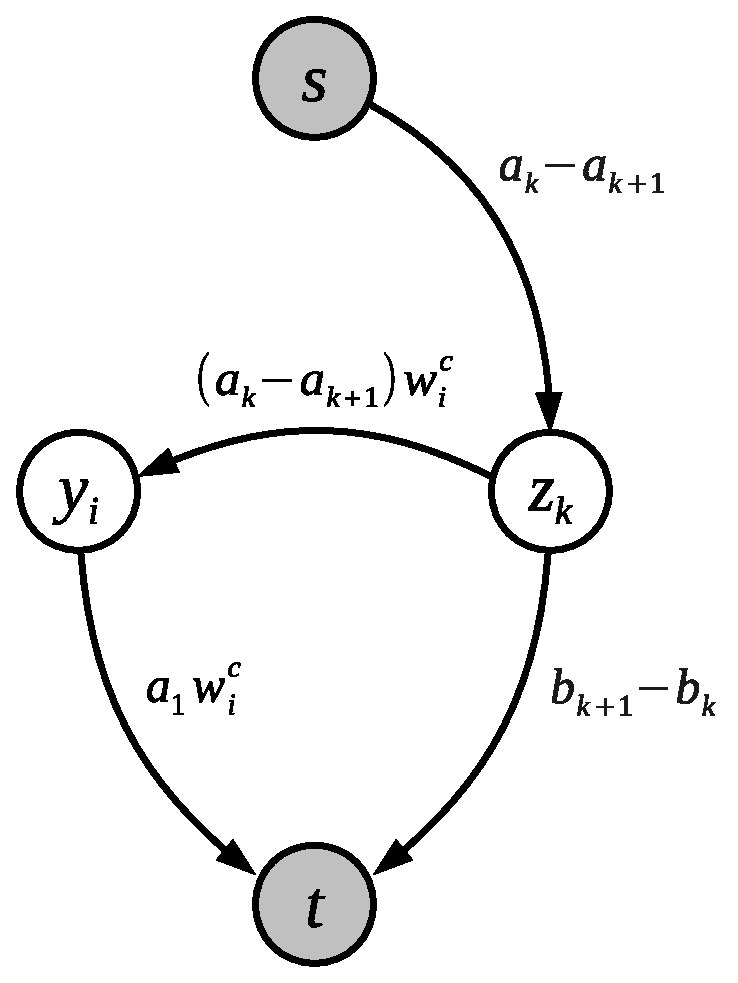
\includegraphics[width=0.55\columnwidth]{figures/stmincut}
  \vspace{2mm}
  \caption{\label{fig:stmincut} Construction of an $st$-graph for
    minimizing energy functions with arbitrary weighted lower linear
    envelope potentials. Every cut corresponds to an assignment to the
    random variables, where variables associated with nodes in the
    ${\cal S}$ set take the value one, and those associated with nodes
    in the $\T$ set take the value zero. With slight abuse of
    notation, we use the variables to denote nodes in our graph. For
    each lower linear envelope potential edges are added as follows:
    for each $i \in c$, add an edge from $y_i$ to $t$ with weight $a_1
    w^c_i$; for each $i \in c$ and $k = 1, \ldots, K-1$, add an edge
    from $z_k$ to $y_i$ with weight $(a_{k} - a_{k+1}) w^c_i$; and for
    $k = 1, \ldots, K-1$, add an edge from $s$ to $z_k$ with weight
    $a_k - a_{k+1}$ and edge from $z_k$ to $t$ with weight $b_{k+1} -
    b_k$.
    %
    Other edges may be required to represent unary and pairwise
    potentials (see \cite{Kolmogorov:PAMI04}).
  }
\end{figure}

Using this fact, we can show that an energy function containing
arbitrary weighted lower linear envelope potentials can be minimized
in polynomial time.

\begin{theorem}
\label{thm:inference}
For binary variables $\by \in \{0, 1\}^n$, let $E^0\!\left(\by\right)$
be a submodular energy function, and let
\[
\energy{\by} = E^0\!\left(\by\right) + \sum_{c \in \C} \psi^H_c\!(\by_c),
\]
where $\psi^H_c\!(\by_c)$ are arbitrary weighted lower linear envelope
higher-order potentials. Then $\energy{\by}$ can be minimized in time
polynomial in the number of variables $n$ and total number of linear
envelope functions.
\end{theorem}
%
\begin{proof}
  By Proposition~\ref{prop:minpsi} we have $\argmin_{\by} E(\by) =
  \argmin_{\by} (E^0\!\left(\by\right) + \sum_c \min_{\bz_c}
  E^c(\by_c, \bz_c))$. By Proposition~\ref{prop:submod} we have that
  the $E^c(\by_c, \bz_c)$ are submodular. The sum of submodular energy
  functions is submodular. Each higher-order term adds $K - 1$
  auxiliary variables so the total number of variables in the
  augmented energy function is less than $n$ plus the total number of
  linear functions.
\end{proof}
\bigskip

\subsection{Relationship to Binary MRFs}

From a graphical models perspective, we note that $E^c(\by_c, \bz_c)$
is nothing more than a pairwise binary Markov random field
(MRF). Evidently, we can express \eqnref{eqn:posiform} as
%
\begin{multline}
  E^c(\by_c, \bz) = \textrm{const.} + \sum_{i \in c} \psi^Y_i\!(y_i) + \sum_{k= 1}^{K-1} \psi^Z_k\!(z_k)\\
  {}+ \sum_{(i,k)} \psi^P_{ik}(y_i, z_k)
  \label{eqn:energy_z}
\end{multline}
%
where, for example, $\psi^Z_k\!(z_k) = \left( b_{k+1} - b_k \right)$
if $z_k = 1$ and $\left( a_k - a_{k+1} \right)$ otherwise. For
brevity, we omit details of the remaining potential functions, which
can be trivially constructed by considering the corresponding unary
and pairwise terms in $y_i$ and $z_k$ between the two forms.

% LEARNING
\section{Learning the Lower Linear Envelope}
\label{sec:learning}

We now show how the max-margin framework can be used to learn
parameters of our weighted lower linear envelope potentials. For
simplicity of exposition we consider a single higher-order term
$\psi^{H}_c(\by_c)$ and drop the subscript $c$ for brevity. The
extension to multiple higher-order terms defined over different
subsets of variables is straightforward.

We begin by reviewing a variant of the max-margin framework introduced
by \citename{Tsochantaridis:ICML04} and \citename{Taskar:ICML05}. We
then show how alternative representations of the weighted lower linear
envelope potential can be learned using the framework.

\subsection{Max-margin Learning}
%
Given an energy function $\energy{\by; \btheta} = \btheta^T \!
\phi(\by)$ parameterized as a linear combination of features
$\phi(\by) \in \reals^m$ and weights $\btheta \in \reals^m$, and a set
of $T$ training examples $\{\by_t\}_{t=1}^T$ the max-margin framework
is a principled approach to learning the weights of the model.

In our formulation we will allow additional linear constraints to be
imposed on the weights of the form $\bG \btheta \geq \bh$, where $\bG
\in \reals^{d \times m}$ and $\bh \in \reals^d$. This is not typically
necessary for max-margin learning, but, as we will see below, is
required for enforcing concavity when learning lower linear envelope
potentials.

Now, let $\Y_t = \{0, 1\}^n$ be the set of all possible assignments
for the $t$-th training example. The (margin-rescaling) max-margin
approach formulates learning as a quadratic programming optimization
problem, $\mmqp{\Y_t}{\bG}{\bh}$:
%
\begin{align}
  & \textrm{minimize} \quad \textstyle \frac{1}{2} \|\btheta\|^2 + \frac{C}{T} \sum_{t=1}^{T} \xi_t
  \label{eqn:maxmarginqp} \\
  & \textrm{subject to} \notag \\
  & \begin{array}{lll}
    & \btheta^T \delta\phi_t(\by) + \xi_t \geq \Delta(\by, \by_t), & \forall t, \by \!\in\! \Y_t, \\
    & \xi_t \geq 0, & \forall t, \\
    & \bG \btheta \geq \bh
  \end{array} \notag
\end{align}
%
where $\delta\phi_t(\by) \triangleq \left(\phi_t(\by) -
\phi_t(\by_t)\right)$ is the difference between feature
representations for some assignment $\by$ and the $t$-th ground-truth
assignment $\by_t$, $C > 0$ is a regularization constant, and
$\Delta(\by, \by_t)$ measures the loss between a ground-truth
assignment $\by_t$ and any other assignment. In our work we use the
Hamming loss, which measures the proportion of variables whose
corresponding assignments disagree. More formally, the Hamming loss is
defined as $\Delta(\by, \by') = \frac{1}{n} \sum_{i=1}^{n} \ind{y_i
  \neq y'_i}$, where $\ind{P}$ is the indicator function taking value
one when $P$ is true and zero otherwise.

The number of constraints in the QP is exponential in the number of
variables, and a standard approach to solving the max-margin QP is by
adding constraints incrementally. Briefly, at each iteration the
algorithm checks for the most violated constraint (for each training
example), using \emph{loss-augmented inference}, and, if found, adds
it to the constraint set. The algorithm terminates when no more
violated constraints are found (see \algref{alg:learning}).

Note that while we use the Hamming loss in this work, the loss
function $\Delta(\by, \by_t)$ in \eqnref{eqn:maxmarginqp} can be more
general. For example, \citet{Pletscher:AISTATS12} recently showed that
certain higher-order losses can be reduced to binary pairwise
supermodular functions. In this way the loss function factors over the
same terms as in the energy function with the addition of auxiliary
variables. Since the loss function is subtracted from the energy
function during loss-augmented inference, the supermodular loss
becomes a submodular objective and therefore admits tractable
minimization.

\subsection{Transforming Between Representations}
\label{sec:representation_transformation}

\begin{figure}[t]
  \centering
  \includegraphics[width=0.9\columnwidth]{figures/concave}
  \caption{\label{fig:concave} Example piecewise-linear concave
    function of $W_{\!c}(\by_c) = \sum_{i \in c} w^c_i y_i$. The
    function can be represented as the minimum over a set of linear
    functions (lower linear envelope) or as a set of sampled points
    $\theta_k$ with curvature constraint.}
\end{figure}

The max-margin formulation (see \eqnref{eqn:maxmarginqp}) requires
that the energy function be expressed as a linear combination of
features and weights, however, our higher-order potential is
represented as the minimum over a set of linear functions. One simple
way to re-parameterize the energy function for learning is to sample
the higher-order potential at regular intervals between zero and one.%
%
\footnote{Recall from \secref{sec:inference} that we have assumed,
  without loss of generality, that $\sum_{i \in c} w^c_i = 1$.}
%
This provides a piecewise linear approximation of the weighted lower
linear envelope and the number of points sampled lets us trade-off
tightness of the approximation with efficiency of inference. Let
$\btheta = (\theta_0, \ldots, \theta_K) \in \reals^{K+1}$ be the
sampled values. Then, we can retrieve the equivalent weighted lower
linear envelope representation as
%
\begin{align}
  a_k &= (\theta_k - \theta_{k-1})K\\
  b_k &= \theta_k - a_k \frac{k}{K} = k \theta_{k-1} - (k - 1) \theta_k
\end{align}
for $k = 1, \ldots, K$ as illustrated in \figref{fig:concave}.%
\footnote{Note that if $a_k = a_{k-1}$ then the $k$-th linear function
  is redundant and can be omitted from the energy function.}
%
The corresponding feature vector $\phi(\by) = \left(\phi_0, \ldots,
\phi_{K}\right) \in \reals^{K+1}$, under this representation, is a
$(K+1)$-length vector with $n$-th entry
%
\begin{align}
  \phi_{n-1} &= \left\{ \begin{array}{ll}
    W(\by) \cdot K - n + 2
    & \textrm{if $\frac{n - 2}{K} \leq W(\by) < \frac{n - 1}{K}$} 
    \\
    n - W(\by) \cdot K
    & \textrm{if $\frac{n - 1}{K} \leq W(\by) < \frac{n}{K}$} 
    \\
    0 & \textrm{otherwise}.
  \end{array} \right.
  \label{eqn:features}
\end{align}
%
so that $\btheta^T \phi(\by)$ linearly interpolates between the
samples corresponding to the active linear function (see
\figref{fig:features}). For example, assume $K = 3$ and $W(\by) =
\frac{1}{2} + \epsilon$ then $\phi(\by) = (0, \frac{1}{2} - 3
\epsilon, \frac{1}{2} + 3 \epsilon, 0)$. Note that $\ones^T \phi(\by)
= 1$. This representation is independent of clique size and so can be
used without modification for applications where clique size varies
between instantiations of the higher-order potentials, \eg when
cliques are derived from superpixels generated from an
over-segmentation algorithm.

\begin{figure}[th]
  \centering
  \includegraphics[width=0.9\columnwidth]{figures/feature_interp}
  \caption{\label{fig:features} Illustration of how the feature vector
    $\phi(\by)$ interpolates between samples to produce the correct
    value for the active linear function.}
\end{figure}

It is instructive to observe that under this representation, with
weighted lower linear envelope sampled at uniform intervals between
$0$ and $1$, we can compute $k^\star = \argmin_{k=1, \ldots, K} \left\{
a_k W(\by) + b_k \right\}$ and hence $\bz$ in closed-form as
%
\begin{align}
  k^\star &= \left\{ \begin{array}{ll}
    1 & \textrm{if $W(\by) = 0$} \\
    \left\lceil W(\by) \cdot K \right\rceil & \textrm{otherwise}
  \end{array} \right.
\end{align}
%
which is the key insight behind the feature representation in
\eqnref{eqn:features}.

We now have a representation of our higher-order potentials which is
linear in the parameters $\btheta$. It remains to ensure that
$\btheta$ represents a concave function. We do this by adding the
second-order curvature constraint $\bD^2 \btheta \geq \zeros$ where
$\bD^2 \in \reals^{(K-1) \times (K+1)}$ is the (negative) discrete
second-derivative operator:
%
\begin{align}
  \bD^2 &= \left[ \begin{matrix}
      -1 & 2 & -1 & 0 & \cdots \\
      & & \ddots \\
      \cdots & 0 & -1 & 2 & -1
    \end{matrix} \right].
\end{align}

Our optimization follows the standard max-margin approach and is
summarized in \algref{alg:learning}.%
%
\footnote{To jointly learn the unary and pairwise weights, we augment
  the parameter vector $\btheta$ with a weight $\theta^\textrm{unary}$
  for the unary terms and non-negative weight $\theta^\textrm{pair}$
  for the pairwise terms, and add the corresponding features
  $\phi^\textrm{unary} = \sum_i \psi^U_i\!(y_i)$ and $\phi^\textrm{pair} =
  \sum_{ij} \psi^P_{ij}(y_i, y_j)$ to the feature vector
  $\phi(\by)$. The non-negativity of $\theta^\textrm{pair}$ ensures
  that the energy function remains submodular.}
%

\begin{theorem}
  For the setting $\epsilon = 0$, \algref{alg:learning} terminates
  with the optimal parameters $\btheta^\star$ for
  $\mmqp{\Y_t}{\bD^2}{\zeros}$.
  \label{thm:learning}
\end{theorem}
%
\begin{proof}
  By Theorem~\ref{thm:inference}, our test for the most violated
  constraints (lines 7 and 8) can be performed exactly ($\Delta(\by,
  \by_t)$ decomposes as a sum of unary terms). If the test succeeds,
  then $\by_t^\star$ cannot already be in $\A_t$. It is now added
  (line 9). Since there are only finitely many constraints, this
  happens at most $2^n - 1$ times (per training example), and the
  algorithm must eventually terminate. On termination there are no
  more violated constraints, hence the parameters are optimal.
\end{proof}
\bigskip

Unfortunately, as our proof suggests, it may take exponential time for
the algorithm to reach convergence with $\epsilon =
0$. \citename{Tsochantaridis:JMLR05} showed, however, that for
$\epsilon > 0$ and no additional linear constraints (\ie $\bG =
\zeros$, $\bh = \zeros$) max-margin learning within a dual
optimization framework will terminate in a polynomial number of
iterations. Their result can be extended to the case of additional
linear constraints (see the Appendix for details).

% ALGORITHM
\begin{algorithm}[tb]
  \begin{algorithmic}[1]
    \STATE{ {\bf input} training set $\{\by_t\}_{t=1}^{T}$, regularization constant $C > 0$,
      and tolerance $\epsilon \geq 0$}
    \STATE{ {\bf initialize} active constraints set $\A_t = \{ \}$ for all $t$}
    \REPEAT

    \STATE{solve $\mmqp{\A_t}{\bD^2}{\zeros}$ to get $\hat{\btheta}$ and
      $\hat{\bxi}$}

    \STATE{convert from $\hat{\btheta}$ to $(a_k, b_k)$ representation}
    \FOR{each training example, $t = 1, \ldots, T$}
    \STATE{compute $\by_t^\star = \argmin_{\by} E(\by; \hat{\btheta}) - \Delta(\by, \by_t)$}
    \IF{$\hat{\xi}_t + \epsilon \!<\! \Delta(\by_t^\star, \by_t) -
      E(\by_t^\star; \hat{\btheta}) + E(\by_t; \hat{\btheta})$}
    \STATE{$\A_t \leftarrow \A_t \cup \{\by_t^\star\}$}
    \ENDIF
    \ENDFOR
    \UNTIL{no more violated constraints}
    \STATE{ {\bf return} parameters $\hat{\btheta}$}
  \end{algorithmic}
  \caption{\label{alg:learning} Learning lower linear envelope MRFs.}
\end{algorithm}

\subsection{Alternative QP Formulations}
\label{sec:alternative_qp}

Our quadratic program above is just one possible formulation that is
based on a particular choice for representing the weighted lower
linear envelope and corresponding feature vectors. An alternative
representation may encode the slope of the weighted lower linear
envelope directly, that is,
%
\begin{align}
  \theta'_i &= \left\{ \begin{array}{ll}
    b_1 & \textrm{for $i = 0$} \\
    a_i = \theta_{i} - \theta_{i-1} & \textrm{for $i = 1, \ldots, K$}
  \end{array} \right.
\end{align}
%

The $i$-th component in the corresponding feature vector is then
$\phi'_i = \sum_{j \geq i} \phi_j$. And instead of a second-order
constraint $\bD^2 \btheta' \geq \zeros$, we have a first-order
constraint $\bD \btheta' \geq \zeros$. Here we can retrieve the $b_k$
recursively as
%
\begin{align}
  b_{k+1} &= (a_k - a_{k+1}) \frac{k}{K} + b_k
  \label{eqn:bk}
\end{align}

One of the advantages of this formulation is that the regularization
term does not penalize flat envelopes (\ie $a_k = 0$). Moreover, it is
interesting to note that under this formulation the optimal
$\theta'_0$ is always zero, \ie $b_1 = 0$, which is not surprising in
light of Observation~\ref{obs:b0}.

We can take this process one step further and represent the
higher-order potential as
%
\begin{align}
  \theta''_k &= \left\{ \begin{array}{ll}
    b_1 & \textrm{for $k = 0$} \\
    a_1 & \textrm{for $k = 1$} \\
    a_{k-1} - a_{k} & \textrm{for $k = 2, \ldots, K$}
  \end{array} \right.
\end{align}
%
with non-negativity constraints on $\theta''_k$ for $k = 2,
\ldots, K$, and appropriate feature vectors, \ie
%
\begin{align}
  \phi''_k &= \left\{ \begin{array}{ll}
    1 & \textrm{if $k = 0$} \\
    W(\by) & \textrm{if $k = 1$} \\
    \left(\frac{(k - 1)}{K} - W(\by)\right)\bigind{W(\by) > \frac{k-1}{K}} & \textrm{$k = 2, \ldots, K$}
  \end{array} \right.
\end{align}

Here we are encoding the coefficients of the pseudo-Boolean function
used during inference directly into the learning problem. Like the
previous formulation we know that the optimal $b_1$ is zero so can
simply drop $\theta_0$ and $\phi_0$ from the optimization.

It is interesting to note the resemblance of the latter QP formulation
with latent-variable structural SVM learning~\cite{Yu:ICML09}. In our
formulation the auxiliary variables $\bz$ (see
\secref{sec:exact_inference}) can be determined directly from the
ground-truth or inferred labels $\by$. Moreover, since we have fixed
the piecewise-linear approximation to have equally spaced
break-points, the auxiliary variables are independent of the
parameters $(a_k, b_k)$ given $\by$. We also have that the $b_k$ are a
function of the $a_k$ (by \eqnref{eqn:bk}). Removing the restriction
of equally spaced break-points (and introducing the $b_k$ into the
optimization) results in a latent-variable SVM. The main difficulty is
that the latent variables $\bz$ now depend on the parameters making
the optimization problem non-convex.

A number of other variants can be considered by linearly constraining
$\btheta$ (or alternatively re-defining $\phi(\by)$). For example, the
parameters of the $P^{n}$-model can be learned by constraining
$\theta_0 \leq \theta_1$ and forcing $\theta_i = \theta_{i-1}$ for $i
= 2, \ldots, K - 1$. Although this case is somewhat uninteresting as
there is only one parameter to learn (since by Observation~\ref{obs:b0}
we can set $\theta_1 = \ldots = \theta_K = 0$ without changing the
shape of the potential function), which can often be done more
efficiently by other means, \eg cross-validation over a range of
values.

% Experiments ----------------------------------------------------------------------
\section{Experimental Results}
\label{sec:experiments}

We conduct experiments on synthetic and real-world data, comparing
baseline MRF models with ones that include higher-order terms learned
by our method.

\subsection{Synthetic Checkerboard}

Our synthetic experiments are designed to explore the different QP
formulations for learning the lower linear envelope model parameters
and provide intuition into the real-world experiments that
follow. They involve an $8 \times 8$ checkerboard pattern of
alternating white ($y_i = 1$) and black ($y_i = 0$) squares. Each
square contains 256 pixels. We associate one variable in the model
with each pixel giving our MRF a total of $8 \times 8 \times 256 =
16,384$ variables. We generate a noisy version of the checkerboard as
input by the following method. Let $\by^\star$ be the ground-truth
checkerboard, then our input is generated as $x_i = \eta_0
\ind{y^\star_i = 0} - \eta_1 \ind{y^\star_i = 1} + \delta_i$ where
$\eta_0$ and $\eta_1$ are the signal-to-noise ratios for the black and
white squares, respectively, and $\delta_i \sim \U(-1, 1)$ is additive
i.i.d.\ uniform noise. Our task is to recover the checkerboard pattern
from the noisy input.

We consider three difference MRF models involving: (i) unary and
pairwise terms, (ii) unary and higher-order terms, and (iii) unary,
pairwise, and higher-order terms. Our unary terms are constructed for
each pixel as $\psi^U_i\!(y_i) = \theta^\textrm{unary} x_i$ where
$\theta^\textrm{unary}$ is an arbitrary weight. The pairwise terms
take the form $\psi^P_{ij}(y_i, y_j) = \theta^\textrm{pair} \ind{y_i
  \neq y_j}$, where $i$ and $j$ are neighbouring pixels, and
$\theta^{\textrm{pair}} \geq 0$ weights the strength of the pairwise
term relative to the unary term.

For models including higher-order terms, we add one lower linear
envelope potential term $\psi^H_c\!(\by_c) = \min_{k=1, \ldots, K}
\left\{ a_k \sum_{i \in c} \frac{1}{|c|} y_i + b_k \right\}$ for each
square in the checkerboard, so each higher-order potential contains
256 variables and the terms are disjoint. Intuitively, we would like
the potential to favour label consistency within the square. We learn
$\theta^{\textrm{unary}}$, $\theta^{\textrm{pair}}$ (when included),
and $\{(a_k, b_k)\}_{k=1}^{K}$ for $K=10$ linear functions using
\algref{alg:learning}. For the baseline model with unary and pairwise
terms we set $\theta^\textrm{unary} = 1$ and choose
$\theta^\textrm{pair}$ to give best the Hamming loss by evaluating 101
uniformly spaced values in the range $[0, 1]$.

We report results on two different problem instances. The first has
symmetric signal-to-noise ratios $\eta_0 = \eta_1 = 0.1$, and the
second has five times less noise on the black squares ($\eta_0 = 0.5$)
than on the white ($\eta_1 = 0.1$). \figref{fig:synthetic_results}
shows the ground-truth checkerboard patterns and the noisy input. For
both instances we set $C = 1000$ in \eqnref{eqn:maxmarginqp}. Learning
is run to convergence, taking 27 iterations for the first instance and
19 iterations for the second instance on the model with unary,
pairwise and higher-order terms. Each training iteration took under 1s
with inference taking about 120ms on a 2.66GHz quad-core Intel CPU.

\figref{fig:synthetic_results} shows the inferred checkerboard
patterns for the pairwise MRF baseline, and for our higher-order model
after the third and after the final training iterations ((c), (d), and
(e), respectively). We see that after just three iterations our
higher-order model is already performing well on both problem
instances, and by the final iteration we can perfectly recover the
checkerboard unlike the pairwise model. This is not surprising given
that our higher-order cliques are defined on the checkerboard
squares. Below we run further experiments with misspecified cliques.

% results
\begin{figure}[t]
  \centering
  \setlength{\tabcolsep}{2pt}
  \begin{tabular}{c|c|c|cc}
    \includegraphics[width=0.18\linewidth]{figures/synthetic/groundtruth} &
    \includegraphics[width=0.18\linewidth]{figures/synthetic/data} &
    \includegraphics[width=0.18\linewidth]{figures/synthetic/pairwise} &
    \includegraphics[width=0.18\linewidth]{figures/synthetic/iteration3} &
    \includegraphics[width=0.18\linewidth]{figures/synthetic/highorder} \\
    {\small (a)} & {\small (b)} &
    {\small (c)} & {\small (d)} &
    {\small (e)}
  \end{tabular}
  \caption{\label{fig:synthetic_results} Inferred output from our
    synthetic experiments. Shown are (a) the ground-truth labels, (b)
    noisy inputs, (c) best inferred labels using a pairwise model,
    (d)-(e) inferred output from the model containing higher-order
    terms after three training iterations and at convergence,
    respectively. Matlab source code for reproducing these results is
    available from the author's homepage.}
\end{figure}

We also compared the shape of the learned lower linear envelope for
different problem instances comparing the different QP formulations
(as described in \secref{sec:alternative_qp}). All formulations were
able to learn parameters that perfectly reconstruct the known
checkerboard pattern. The learned linear envelope parameters (relative
to the unary weight) are shown in \figref{fig:synthetic_weights}. Note
that for the second instance (with asymmetric noise), our algorithm is
able to learn an asymmetric potential.

\begin{figure*}[t]
  \centering
  \setlength{\tabcolsep}{2pt}
  \begin{tabular}{ccc}
    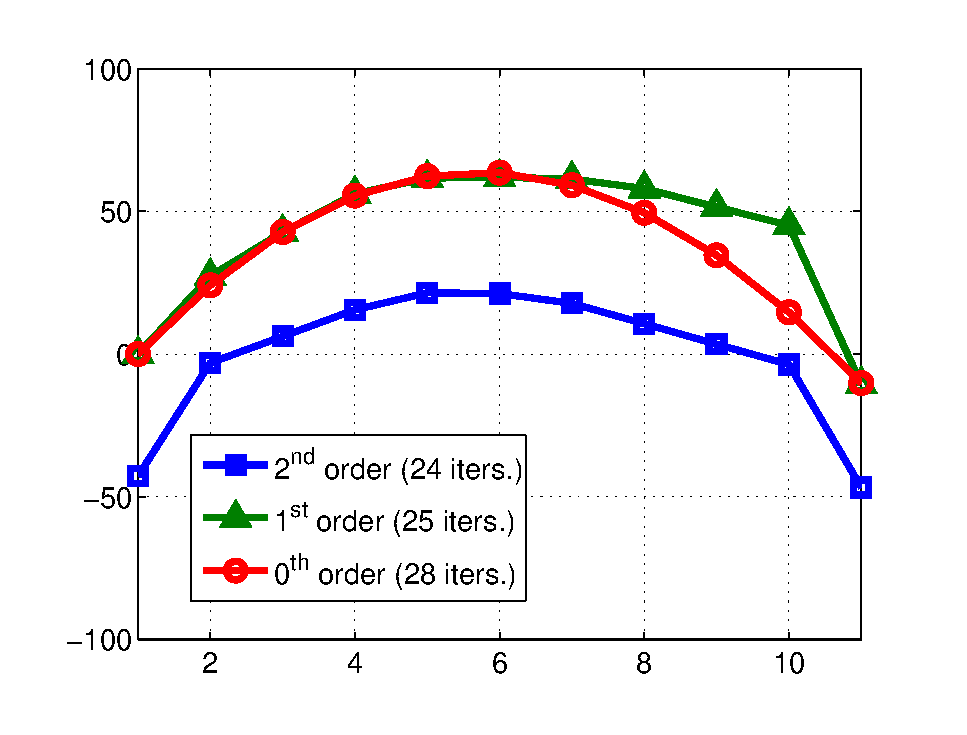
\includegraphics[width=0.32\linewidth]{figures/synthenv1} &
    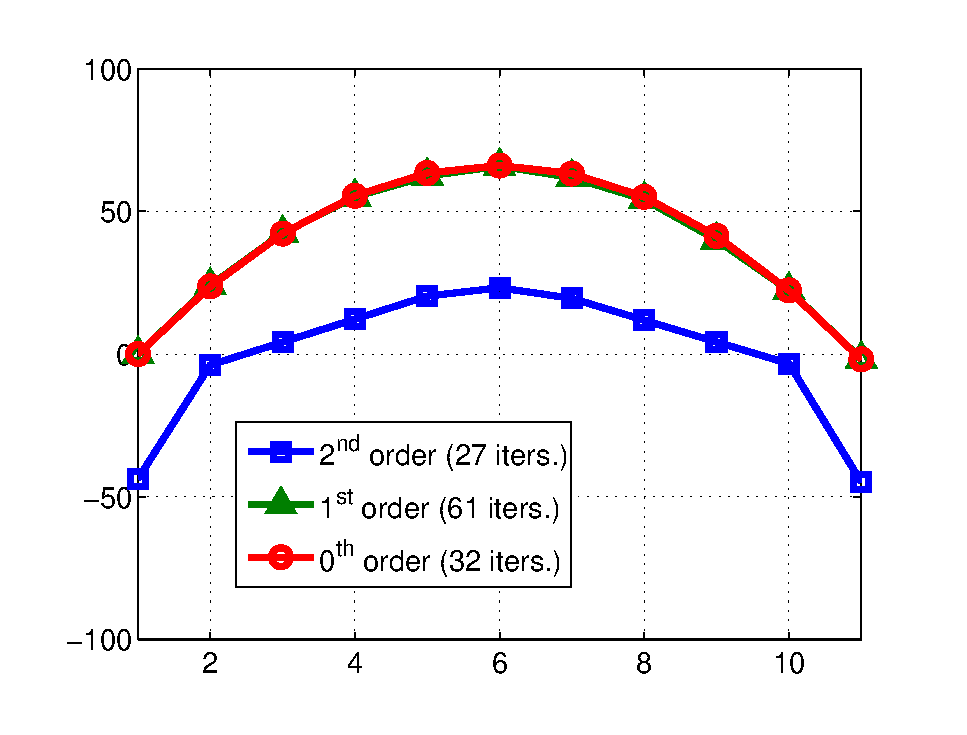
\includegraphics[width=0.32\linewidth]{figures/synthenv5} &
    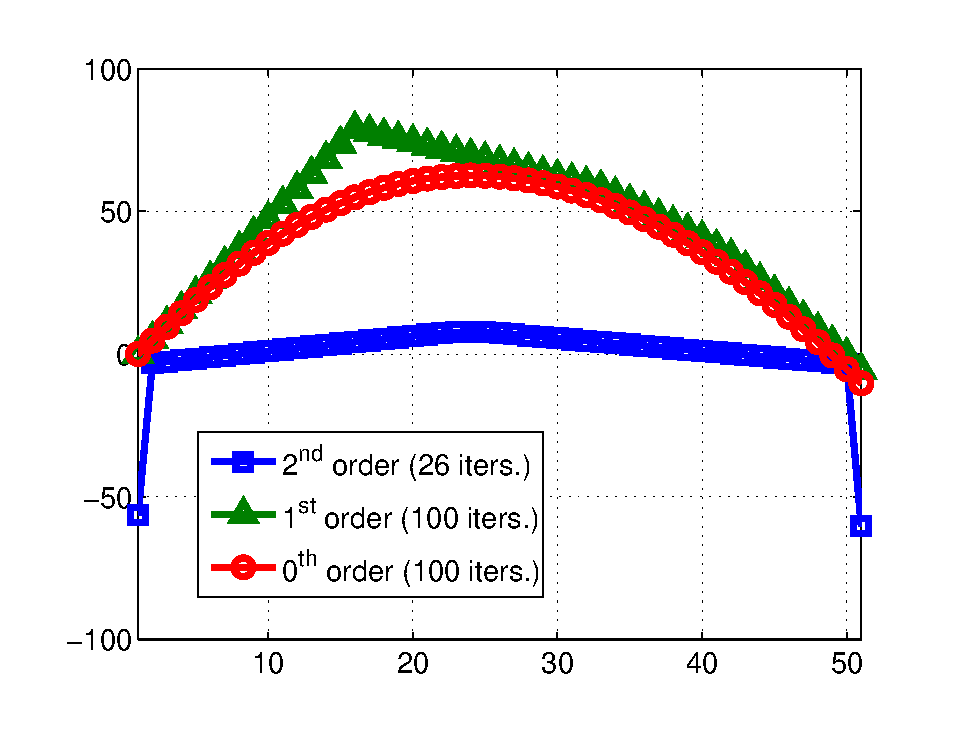
\includegraphics[width=0.32\linewidth]{figures/synthenv2} \\
    {\small (a)} & {\small (b)} & {\small (c)} \\
    \includegraphics[width=0.32\linewidth]{figures/synthenv3} &
    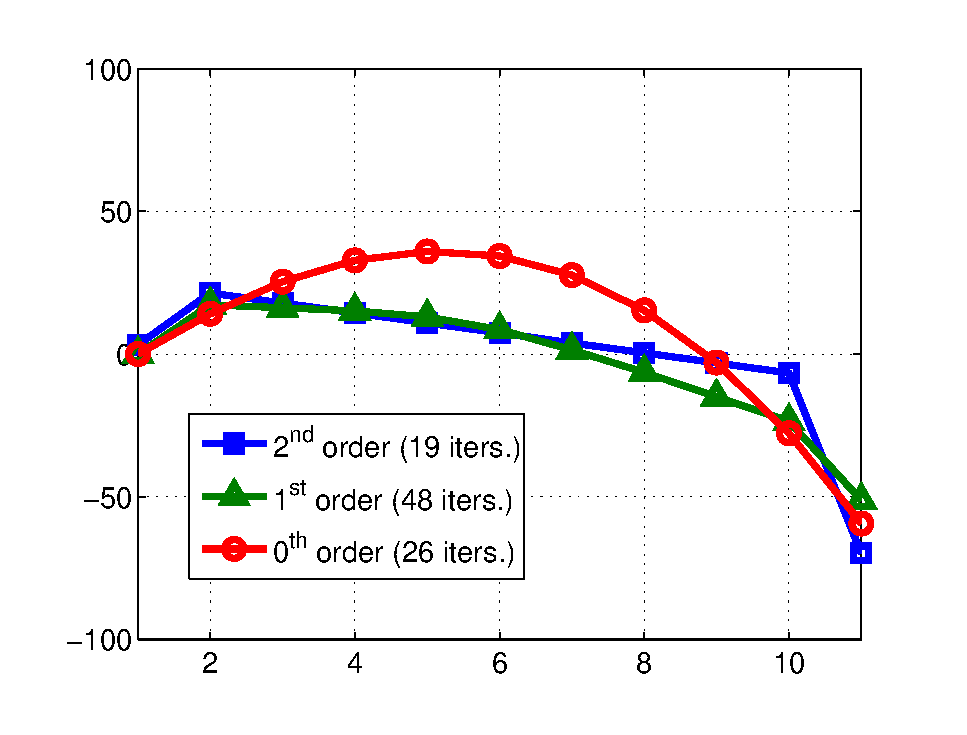
\includegraphics[width=0.32\linewidth]{figures/synthenv6} &
    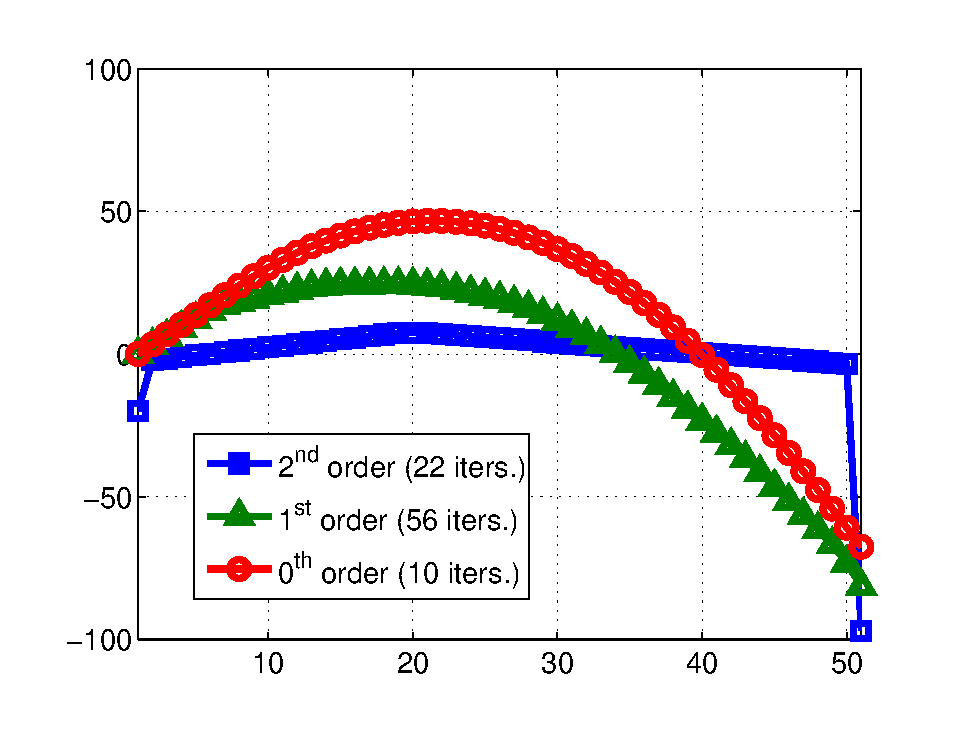
\includegraphics[width=0.32\linewidth]{figures/synthenv4} \\
    {\small (d)} & {\small (e)} & {\small (f)}
  \end{tabular}
  \caption{\label{fig:synthetic_weights} Learned linear envelopes
    (parameters are normalized by the unary weight) for synthetic
    experiments. The first row (a)-(c) shows results with symmetric
    noise ($\eta_0 = \eta_1 = 0.1$) while the second row (d)-(f) shows
    results with asymmetric noise ($\eta_0 = 0.5$ and $\eta_1 =
    0.1$). Compared are models with unary and higher-order potentials
    with $K = 10$ linear terms ((a) and (d)), unary, pairwise and
    higher-order potentials ((b) and (e)), and unary and higher-order
    potentials with $K = 50$ linear terms ((c) and (f)).}
\end{figure*}

Next we evaluate our algorithm on synthetic data with partially
overlapping as well as misspecified cliques. Here we generate multiple
cliques (between one and five) for each checkerboard square then
randomly remove between 5\% and 50\% of the pixels from each
clique. We also introduce a number of completely misspecified cliques
composed of pixels chosen at random from anywhere in the image---on
expectation half the pixels in these cliques have ground-truth label
one and half have ground-truth label zero. We learn a model with unary
and higher-order terms only.

Inferred checkerboard patterns are shown in
\figref{fig:synth_corrupt_results}. Increasing from left to right is
the percentage of pixels randomly removed from the cliques (\ie
reduction in clique size). Increasing from top to bottom is the number
of overlapping cliques. As expected our model performs poorly when
many of the pixels are not covered by a higher-order clique, for
example in \figref{fig:synth_corrupt_results}(i)(d). Multiple
partially overlapping cliques addresses this problem. Moreover, our
method is robust to a reasonable number of misspecified cliques (10\%
in the case of the results shown in \figref{fig:synth_corrupt_results}).

\begin{figure}[t]
  \centering
  \setlength{\tabcolsep}{2pt}
  \begin{tabular}{ccccc}
    \small {(i)} & 
    \includegraphics[width=0.18\linewidth]{figures/synth_corrupt/synth_corrupt_1_1} &
    \includegraphics[width=0.18\linewidth]{figures/synth_corrupt/synth_corrupt_1_2} &
    \includegraphics[width=0.18\linewidth]{figures/synth_corrupt/synth_corrupt_1_3} &
    \includegraphics[width=0.18\linewidth]{figures/synth_corrupt/synth_corrupt_1_4} \\
    \small {(ii)} & 
    \includegraphics[width=0.18\linewidth]{figures/synth_corrupt/synth_corrupt_2_1} &
    \includegraphics[width=0.18\linewidth]{figures/synth_corrupt/synth_corrupt_2_2} &
    \includegraphics[width=0.18\linewidth]{figures/synth_corrupt/synth_corrupt_2_3} &
    \includegraphics[width=0.18\linewidth]{figures/synth_corrupt/synth_corrupt_2_4} \\
    \small {(iii)} & 
    \includegraphics[width=0.18\linewidth]{figures/synth_corrupt/synth_corrupt_3_1} &
    \includegraphics[width=0.18\linewidth]{figures/synth_corrupt/synth_corrupt_3_2} &
    \includegraphics[width=0.18\linewidth]{figures/synth_corrupt/synth_corrupt_3_3} &
    \includegraphics[width=0.18\linewidth]{figures/synth_corrupt/synth_corrupt_3_4} \\
    & {\small (a)} & {\small (b)} & {\small (c)} & {\small (d)}
  \end{tabular}
  \caption{\label{fig:synth_corrupt_results} Inferred output from our
    synthetic experiments with misspecified cliques. Shown are
    inferred outputs from the model at convergence. Rows (i)--(ii)
    correspond to partially covering each grid square with 1, 2 and 5
    higher-order cliques, respectively. Columns (a)-(d) correspond to
    the size of each clique (95\%, 90\%, 75\%, 50\% grid square
    coverage, respectively). In addition, 10\% of the cliques were
    generated to contain random a random mix of pixels.}
\end{figure}


\subsection{Interactive Figure-Ground Segmentation}

We also ran experiments on the real-world ``GrabCut'' problem
introduced by~\citename{Rother:SIGGRAPH04}. Here the aim is to segment
a foreground object from an image given a user-annotated bounding box
of the object (see \figref{fig:grabcut_results}(a) for some
examples). To solve this problem the GrabCut algorithm associates a
binary random variable $y_i$ with each pixel in the image indicating
whether the pixel belongs to the ``background'' (binary label 0) or
the ``foreground'' (binary label 1). Variables corresponding to pixels
outside of the user-annotated bounding box are automatically assigned
a label of zero (\ie background). The assignment for the remaining
variables, \ie those within the bounding box, is inferred.

We compare a model with learned higher-order terms against the
baseline GrabCut model by performing leave-one-out cross-validation on
a standard set of 50 images
from~\citename{Lempitsky:ICCV09}. Following the approach of
\citename{Rother:SIGGRAPH04}, our baseline model contains unary and
pairwise terms. The unary terms are defined as the log-likelihood from
foreground and background Gaussian mixture models (GMMs) over pixel
colour and are image-specific. Briefly, the GMMs are initialized by
learning foreground and background models from pixels inside and
outside the user-annotated bounding box, respectively. Next, the GMMs
are used to relabel pixels (within the bounding box) as either
foreground or background by taking the label with highest likelihood
according to the current parameter settings. Next the parameters of
the foreground and background colour models are re-estimated given the
new labeling. This process of parameter estimation and re-labeling is
repeated until convergence (or a maximum number of iterations is
reached). The final GMMs are used to construct the unary terms.

The pairwise terms encode smoothness between each pixel and its eight
neighbours, and are defined as
%
\begin{align}
  \psi^P_{ij}(y_i, y_j) &= \frac{\lambda}{d_{ij}} \ind{y_i \neq y_j} \exp\left\{- \frac{\|x_i - x_j\|^2}{2 \beta}\right\}
\end{align}
%
where $d_{ij}$ is the distance between pixels $i$ and $j$, $x_i$ and
$x_j$ are the RGB colour vectors for pixels $i$ and $j$, $\beta$ is
the average squared-distance between adjacent RGB colour vectors in
the image, and $\lambda$ determines the strength of the pairwise
smoothness term. It is the only free parameter in the baseline model
and learned by cross-validation.

To construct the higher-order terms, we adopt a similar
superpixel-based approach to~\citename{Ladicky:ICCV09}. First, we
over-segment the image into a few hundred superpixels. Here we use the
mean-shift segmentation algorithm of~\citename{Comaniciu:PAMI02} but
our method does not depend on this choice. The pixels within each
superpixel then define a higher-order term, much like the checkerboard
squares in our synthetic experiments. Here, however, the higher-order
terms are over different sized cliques and there is no guarantee that
they should be labeled homogeneously.

We learn the weights for the unary and pairwise potentials and the
parameters for a lower linear envelope potential with $K = 10$ terms
using \algref{alg:learning}. We set $C = 1000$ and ran for a maximum
of 100 iterations, however, for most cross-validation folds, the
algorithm converged before the maximum number of iterations was
reached. The parameters determined at the last iteration were used for
testing. Learning took approximately 3 hours per cross-validation fold
with the majority of the time spent generating violated constraints
for the 49 training images (each typically containing $640\times480$
pixels).

Some example results are shown in \figref{fig:grabcut_results}. The
first row shows that our higher-order terms can capture some fine
structure such as the cheetah's tail but it also segments part of the
similarly-appearing rock. In the second example, we are able to
correctly segment the person's legs. The third example shows that we
are able to segment the petals at the lower part of the rightmost
flower, which the baseline model does not. The final example (fourth
row) shows that our model is able to remove background regions that
have similar appearance to the foreground. However, we can also make
mistakes such as parts of the sculpture's robe. Quantitatively, our
method achieves 91.5\% accuracy compared to 90.0\% for the strong
baseline.

% grabcut results
\begin{figure}[t]
  \begin{center}
      \begin{tabular}{c}
        \begin{tabular}{p{0.24\linewidth}p{0.24\linewidth}p{0.24\linewidth}p{0.24\linewidth}}
          {\small \hspace{5mm} (a)} & 
          {\small \hspace{6.5mm} (b)} &
          {\small \hspace{8mm} (c)} & 
          {\small \hspace{9mm} (d)}
        \end{tabular}
    \end{tabular}
    \caption{\label{fig:grabcut_results} Example results from our
      GrabCut experiments. Shown are: (a) the image and bounding box,
      (b) ground-truth segmentation, (c) baseline model output, and
      (d) output from model with higher-order terms.}
  \end{center}
\end{figure}

\subsection{Weizmann Horses}

We also ran experiments on the 328-image Weizmann Horse
dataset~\cite{Borenstein:ECCV02, Borenstein:CVPR04}. The task here is
a supervised machine learning one with the goal being to segment
horses from the background in unseen images. As with the previous
experiments, our model consists of unary, pairwise and higher-order
lower linear envelope terms.

We divide the dataset into three subsets of size 100, 64 and 164. The
first subset of 100 images is used to learn a classifier for
predicting horse pixels from local features. The second subset of 64
images is used to learn the weights for the unary and pairwise terms,
and the parameters of the higher-order lower linear envelope
potentials. The final subset of 164 images is used for testing.

Concretely, our unary terms contain the log-probability from a
learned boosted decision tree classifier, which estimates the
probability of each pixel belonging to a horse given colour and
texture features surrounding the pixel. We use the 17-dimensional
``texton'' filterbank of \citename{Shotton:ECCV06} for describing
texture.

Again for the higher-order terms we over-segment the images using the
mean-shift segmentation algorithm~\cite{Comaniciu:PAMI02} to produce
superpixels. However, instead of a single over-segmentation we compute
multiple over-segmentations by varying the spatial and colour
bandwidth parameters of the mean-shift algorithm. Superpixels
containing less than 64 pixels are discarded. The remaining set of
(overlapping) superpixels are used to define cliques for the
higher-order terms with $K = 10$ linear functions.

Training the boosted classifier on the colour and texture features for
the unary potentials took approximately 7 minutes on a 2.66GHz
quadcore Intel CPU. Cross-validating the strength of the pairwise term
for the model without higher-order terms took a further 15
minutes. When training the model with higher-order terms we learn all
parameters simultaneously. This took approximately 6 hours with the
bulk of the time spent running loss-augmented inference.

We compare a baseline model with unary and pairwise terms against a
model that also includes the lower linear envelope potentials. Results
showing average pixel accuracy over the set of test images are shown
in \tabref{tab:weizmann_results}. Once again the baseline model is
very strong but our method with higher-order terms is able to achieve
a slight improvement.

\begin{table}
  \normalsize
  \centering
  \begin{tabular}{|l|c|}
    \hline
    {\sc Model} & {\sc Accuracy} \\
    \hline \hline
    Baseline & 90.9 \\
    \hline
    Higher-Order (1 Seg.) & 91.4 \\
    Higher-Order (2 Segs.) & {\bf 91.6} \\
    Higher-Order (3 Segs.) & 91.2 \\
    \hline
  \end{tabular}
  \caption{\label{tab:weizmann_results} Results from our Weizmann
    Horse experiments. The baseline model includes unary and pairwise
    terms. The higher-order model includes unary, pairwise and
    lower-linear envelope terms defined by multiple
    over-segmentations. See text for details.}
\end{table}

Example horse/background segmentation results are shown in
\figref{fig:weizmann_results}. Qualitatively our method performs
better than the baseline on regions where the contrast between the
foreground horse and background is low (\eg~in the third row of
\figref{fig:weizmann_results}). This is not surprising when we consider
that low contrast boundaries are exactly where the pairwise smoothness
term is expected to perform poorly.

% weizmann results
\begin{figure}[t]
  \begin{center}
    \setlength{\tabcolsep}{0pt}
    \includegraphics[width=\linewidth]{figures/weizmann/horse165} \\
    \vspace{1mm}
    \includegraphics[width=\linewidth]{figures/weizmann/horse232} \\
    \vspace{1mm}
    \includegraphics[width=\linewidth]{figures/weizmann/horse239} \\
    \vspace{1mm}
    \includegraphics[width=\linewidth]{figures/weizmann/horse250} \\
    \vspace{1mm}
    \includegraphics[width=\linewidth]{figures/weizmann/horse268} \\
    \vspace{1mm}
    \includegraphics[width=\linewidth]{figures/weizmann/horse276} \\
      \begin{tabular}{c}
        \begin{tabular}{p{0.2\linewidth}p{0.2\linewidth}p{0.2\linewidth}p{0.2\linewidth}p{0.2\linewidth}}
          {\small \hspace{5.5mm} (a)} & 
          {\small \hspace{6mm} (b)} &
          {\small \hspace{6mm} (c)} & 
          {\small \hspace{6mm} (d)} &
          {\small \hspace{6mm} (e)}
        \end{tabular}
    \end{tabular}
    \caption{\label{fig:weizmann_results} Example segmentations
      produced by our Weizmann Horse experiments. Shown are: (a) the
      image, (b) baseline foreground mask, (c) baseline model
      foreground overlay, (d) higher-order model foreground mask, and
      (e) higher-order model foreground overlay.}
  \end{center}
\end{figure}


% Discussion -----------------------------------------------------------------------
\section{Discussion}
\label{sec:discussion}

This paper has shown how to perform efficient inference and learning
for lower linear envelope binary MRFs, which are becoming popular for
enforcing higher-order consistency constraints over large sets of
random variables, particularly in computer vision.

Our formulation allows arbitrary non-negative weights to be assigned
to each variable in the higher-order term. These weights allow
different size cliques to share the same higher-order parameters
(resulting in the same shape lower linear envelope). In addition, the
weights can be used to place more importance on some variables than
others, \eg pixels further away from the boundary of a superpixel.

Our work suggests a number of directions for future research. Perhaps
the most obvious is extending our approach to multi-label MRFs. An
initial exploration of this extension was done by
\citename{Park:ECCV2012} using our inference method within the inner
loop of move-making algorithms such as $\alpha$-expansion or
$\alpha\beta$-swap~\cite{Boykov:ICCV99} for generating
constraints. However, the question of efficient learning remains open
since inference in this regime is only approximate.

Other straightforward extensions include the introduction of features
for modulating the higher-order terms and the use of dynamic graph
cuts~\cite{Kohli:PAMI07} for accelerating loss-augmented inference
within our learning framework. We could also consider other
optimization schemes for solving our learning problem, \eg
dual-decomposition~\cite{Komodakis:CVPR2011} or the subgradient
method~\cite{Nowozin:2011, Bertsekas:2004}.

More interesting is the implicit relationship between structured
higher-order models and latent-variable SVMs~\cite{Yu:ICML09} as
suggested by the introduction of auxiliary variables for inference and
our alternative QP formulations. Exploring this relationship further
may provide insights into both models.

From an application perspective, we hope that the ability to
efficiently learn higher-order potentials from data will encourage
researchers to more readily adopt these more expressive models for
their applications.

% Acknowledgments -----------------------------------------------------------------

\section*{Acknowledgments}
This research was supported under Australian Research Council's
\emph{Discovery Projects} funding scheme (project number DP110103819).


% Bibliography --------------------------------------------------------------------

{
  \bibliographystyle{abbrvnat}
%  \bibliographystyle{unsrtnat}
  \bibliography{long,scene}
}

% Biography -----------------------------------------------------------------------

\begin{IEEEbiography}[{\includegraphics[width=1in,height=1.25in,clip,keepaspectratio]{figures/sgould_bw}}]{Stephen Gould}
is a Fellow in the Research School of Computer Science in the College
of Engineering and Computer Science at the Australian National
University. He received his BSc degree in mathematics and computer
science and BE degree in electrical engineering from the University of
Sydney in 1994 and 1996, respectively. He received his MS degree in
electrical engineering from Stanford University in 1998. He then
worked in industry for a number of years before returning to PhD
studies in 2005. He earned his PhD degree from Stanford University in
2010. His research interests are in computer and robotic vision,
machine learning, probabilistic graphical models, and optimization. He
is a member of the IEEE.
\end{IEEEbiography}

% Appendix ------------------------------------------------------------------------
\clearpage
\appendix

In this section we show that the polynomial time cutting-plane method
of \citename{Tsochantaridis:JMLR05} can be extended to handle linear
inequality constraints on the parameters. Our argument follows their
$\text{SVM}_1^{\Delta m}$ formulation of the max-margin structured
prediction problem.

Let us begin by writing out the Lagrangian for the quadratic program
$\mmqp{\Y_t}{\bG}{\bh}$  defined in Equation 8.
Introducing dual variables $\balpha$, $\bbeta$ and $\bgamma$, we have
%
\begin{multline}
  \Ell(\btheta, \bxi, \balpha, \bbeta, \bgamma) =
  \frac{1}{2} \|\btheta\|^2 + \frac{C}{T} \sum_{t=1}^{T} \xi_t\\
  {}- \sum_{t=1}^{T} \sum_{\by \in \Y_t} \alpha_{t, \by} \left(\btheta^T \delta\phi_t(\by) + \xi_t - \Delta(\by, \by_t)\right)\\
  {}- \bbeta^T \left( \bG \btheta - \bh\right) - \sum_{t=1}^T \gamma_t \xi_t
  \label{eqn:lagrangian}
\end{multline}
%
subject to $\balpha \succeq \zeros$, $\bbeta \succeq \zeros$, and
$\bgamma \succeq \zeros$ where ``$\ba \succeq \bb$'' denotes
componentwise inequality between the vectors $\ba$ and $\bb$.

Setting $\frac{\partial \Ell}{\partial \xi_i} = \frac{C}{T} -
\sum_{\by \in \Y_t} \alpha_{t,\by} - \gamma_t = 0$ and substituting
for $\gamma_t$ we can re-write \eqnref{eqn:lagrangian} as
%
\begin{multline}
  \Ell(\btheta, \balpha, \bbeta) =
  \frac{1}{2} \|\btheta\|^2 \\
  {}- \sum_{t=1}^{T} \sum_{\by \in \Y_t} \alpha_{t, \by} \left(\btheta^T \delta\phi_t(\by) - \Delta(\by, \by_t)\right)\\
  {}- \bbeta^T \left( \bG \btheta - \bh\right)
  \label{eqn:lagrangian2}
\end{multline}
%
subject to constraints $\sum_{\by \in \Y_t} \alpha_{t,\by} \leq
\frac{C}{T}$ for all $t = 1, \ldots, T$.

Now
\begin{align}
\nabla_{\btheta} \Ell 
&= \btheta - \sum_{t=1}^T \sum_{\by \in \Y_t} \alpha_{t,\by} \delta\phi_t(\by) - \bG^T\bbeta.
\end{align}
%
Eliminating $\btheta$ by setting $\nabla_{\btheta} \Ell = 0$ we have
%
\begin{multline}
  \Ell(\balpha, \bbeta) =
  -\frac{1}{2} \sum_{\substack{t=1,\\\by \in \Y_t}}^{T} \sum_{\substack{t'=1,\\\by' \in \Y_t'}}^{T}
  \alpha_{t, \by} \alpha_{t', \by'} \delta\phi_t(\by)^T \delta\phi_{t'}(\by') \\
  - \sum_{\substack{t=1,\\\by \in \Y_t}}^{T} \alpha_{t, \by} \delta\phi_t(\by)^T \bG^T \bbeta
  -\frac{1}{2} \bbeta^T \bG \bG^T \bbeta \\
  + \sum_{\substack{t=1,\\\by \in \Y_t}}^{T} \alpha_{t, \by} \Delta(\by, \by_t) + \bh^T \bbeta\
  \label{eqn:lagrangian3}
\end{multline}
%
where we have written the double summations over $t$ and $\by$ more
succinctly. This is a quadratic equation that can be written more
compactly as
%
\begin{align}
  \Ell(\balpha, \bbeta) &=
  -\frac{1}{2} \begin{bmatrix}\balpha \\ \bbeta \end{bmatrix}^T 
  \!\! \begin{bmatrix}\bJ_{\alpha\alpha} & \bJ_{\alpha\beta} \\ \bJ_{\beta\alpha} & \bG\bG^T \end{bmatrix}
  \! \begin{bmatrix}\balpha \\ \bbeta \end{bmatrix} +
  \begin{bmatrix} \bDelta \\ \bh \end{bmatrix}^T \!\! \begin{bmatrix}\balpha \\ \bbeta \end{bmatrix}
  \label{eqn:lagrangian_matrix}
\end{align}
%
where $\balpha$ is a vector containing the $\alpha_{t,\by}$, $\bDelta$
is a vector with entries $\Delta(\by, \by_t)$ corresponding to the
entries in $\balpha$.

The dual optimization problem to $\mmqp{\Y_t}{\bG}{\bh}$ is to
maximize $\Ell(\balpha, \bbeta)$ subject to constraints $\balpha
\succeq \zeros$, $\bbeta \succeq \zeros$, and $\sum_{\by \in \Y_t}
\alpha_{t,\by} \leq \frac{C}{T}$ for $t = 1, \ldots, T$.

Lemmas 10, 11, 12, and 13 from \citename{Tsochantaridis:JMLR05} apply
directly to \eqnref{eqn:lagrangian3} on the joint variables $(\balpha,
\bbeta)$. Specifically, we have the following bounds
%
\begin{multline}
  \max_{0 < \lambda \leq D} \{\Ell(\hat{\balpha} + \lambda \eta, \hat{\bbeta})\} 
  - \Ell(\hat{\balpha}, \hat{\bbeta}) 
  \\
  \geq \frac{1}{2} \min \left\{D, 
  \frac{\eta^T \nabla_{\alpha} \Ell(\hat{\balpha}, \hat{\bbeta})}{\eta^T \bJ_{\alpha\alpha} \eta}
  \right\} \eta^T \nabla_{\alpha} \Ell(\hat{\balpha}, \hat{\bbeta})
\end{multline}
%
and
%
\begin{multline}
  \max_{0 < \lambda \leq D} \{\Ell(\hat{\balpha} + \lambda \be_{t,\by}, \hat{\bbeta})\} 
  - \Ell(\hat{\balpha}, \hat{\bbeta}) 
  \\
  \geq \frac{1}{2} \min \left\{D, 
  \frac{\frac{\partial \Ell}{\partial \alpha_{t,\by}}(\hat{\balpha}, \hat{\bbeta})}{\|\delta \phi_t(\by)\|^2} 
  \right\}
  \frac{\partial \Ell}{\partial \alpha_{t,\by}}(\hat{\balpha}, \hat{\bbeta})
\end{multline}
%
from Lemmas 12 and 13, respectively.

%\algref{alg:learning}

Now for a given pair of primal parameters $(\hat{\btheta},
\hat{\bxi})$ and corresponding dual variables $(\hat{\balpha},
\hat{\bbeta})$, consider the adding an example $\by_t^\star$ to the
constraint set $\A_t$ in Line 9 of Algorithm~1. Fixing $\bbeta =
\hat{\bbeta} \geq \zeros$ we can write
%
\begin{multline}
  \Ell(\balpha; \hat{\bbeta}) =
  -\frac{1}{2} \sum_{\substack{t=1,\\\by \in \Y_t}}^{T} \sum_{\substack{t'=1,\\\by' \in \Y_t'}}^{T}
  \alpha_{t, \by} \alpha_{t', \by'} \delta\phi_t(\by)^T \delta\phi_{t'}(\by') \\
  + \sum_{\substack{t=1,\\\by \in \Y_t}}^{T} \alpha_{t, \by} \left(\Delta(\by, \by_t) - \delta\phi_t(\by)^T \bG^T \hat{\bbeta} \right) + \kappa(\hat{\bbeta})
\end{multline}
%
where $\kappa$ is independent of $\balpha$. Then recognizing that
%
\begin{align}
  \hat{\btheta} &= \sum_{\substack{t=1,\\\by \in \Y_t}}^{T} \hat{\alpha}_{t, \by} \delta\phi_t(\by)^T + \bG^T \hat{\bbeta}
\end{align}
%
and
%
\begin{align}
  \Delta(\by^\star_t, \by_t) - \hat{\btheta}^T\delta\phi_t(\by_t^\star)
  \,>\, \hat{\xi}_t + \epsilon \,\geq\, \epsilon
\end{align}
% 
we arrive at the same bound for improvement in $\Ell$ as
[Proposition 17, 34] for $\text{SVM}_1^{\Delta
  m}$.

Finally, noticing that for the case of $\bh = \zeros$ we have as a
primal feasible point $\btheta = \zeros$.  Therefore we can upper
bound $\Ell(\balpha, \bbeta)$ by $C \bar{\Delta}$ where $\bar{\Delta}
= \max_{t,\by \in \Y_t} \Delta(\by, \by_t)$ and so Theorem 18, which
bounds the number of iterations of the dual optimization algorithm of
\citename{Tsochantaridis:JMLR05}, applies. We conclude that for
$\epsilon > 0$ our algorithm will converge in a polynomial number of
iterations.

\end{document}
